\documentclass[11pt,a4paper]{report}
\usepackage[utf8]{inputenc}
\usepackage[margin=0.8in]{geometry}
\usepackage{graphicx}
\usepackage[normalem]{ulem}
\useunder{\uline}{\ul}{}
\begin{document}
\begin{center}
\section*{Assignment No. 3}
\end{center}
\rule{\textwidth}{1pt}
\textbf{Aim:}Use of divide and conquer strategies to exploit distributed/parallel/concurrent processing of the above to identify objects,morph-isms, overloading in functions (if any), and functional relations and any other dependencies (as per requirements).\\
\rule{\textwidth}{1pt}
\section*{Divide and Conquer Strategies:}
\paragraph{}In computer science, divide and conquer is an algorithm design paradigm based on multi-branched recursion. A divide and conquer algorithm works by recursively breaking down a problem into two or more sub-problems of the same or related type, until these become simple enough to be solved directly. The solutions to the sub-problems are then combined to give a solution to the original problem. Divide-and-conquer is probably the best-known general algorithm design technique. Though its fame may have something to do with its catchy name, it is well deserved Quite a few very efficient algorithms are specific implementations of this general strategy.\\

\textbf{Divide and conquer algorithms work according to the following general plan:\\}
1. A problem is divided into several sub-problems of the same type, ideally of about equal size.\\
2. The sub-problems are solved (typically recursively, though sometimes a different algorithm is employed, especially when sub-problems become small enough).\\
3. If necessary, the solutions to the sub-problems are combined to get a solution to the original problem.\\

\begin{figure}[ht]
	\centering
	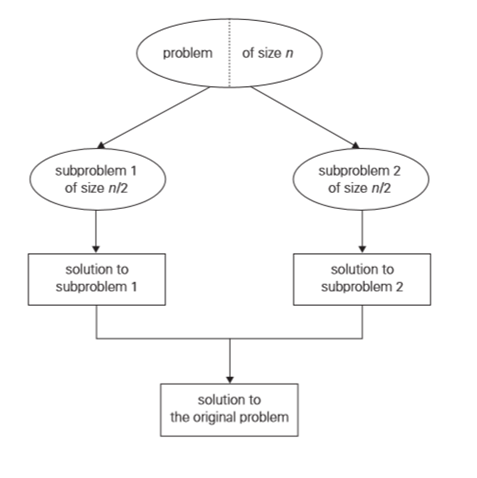
\includegraphics[width=5in]{divc.png}
	\begin{center}\caption{Divide and Conquer Strategies} \end{center}
	\label{LABEL}
\end{figure}
\textbf{Morph-isms:\\}
\textbf{1. Set Theory:\\}
System S is denoted as collection of following set:\\
S = \{Ip, Op, Su\}\\
\begin{table}[h]
\centering
\begin{tabular}{|l|l|l|}
\hline
Mapping Functions f(x) & X   & Y   \\ \hline
F2(Ip1) Ý Op1          & Ip1 & Op1 \\ \hline
F3(Ip1) Ý Op2          & Ip2 & Op2 \\ \hline
F4(Op2) Ý Op3          & Op2 & Op3 \\ \hline
F6(Ip2) Ý Su           & Op2 & Su  \\ \hline
\end{tabular}
\end{table}
\textbf{2. Objects:\\}
\textbf{Inputs:\\}
(a)	Input1: Ip1 = \{Username, Password\}\\
(b)	Input2 : Ip2= \{File Selection\}\\
\newline
\textbf{Outputs:\\}
(a)	Output1 : Op1 = \{Incoming file notification\}\\
(b)	Output2 : Op2 = \{File receiving operation\}\\
(c) Output3 : Op3 = \{Successful write of file in memory\}\\
\textbf{\\Functional Dependency Graph:\\}
(a)	Function 1 = F1 = Collect username and password\\
(b)	Function 2 = F2 = Select file \\
(c)	Function 3 = F3 = Load file in byte array\\
(d)	Function 4 = F4 = Start transmission\\
(e)	Function 5 = F5 = Start file receiving\\
(f)	Function 6 = F6 = View output\\

\end{document}